\chapter{Implementace}

V této části bakalářské práce se zaměříme na praktickou implementaci evolučních algoritmů. Kromě toho je nutné ale i implementovat fyzikální prostředí, podobné tomu jako je ve hře polybridge. V první řadě se zaměříme aby se naše simulace co nejvěrněji podobala hře, což umožní použít řešení navrhnuté evolučními algoritmy i ve hře. Nasledně navrhneme několik různých podob evolučních algoritmů pro stavbu mostu a ty mezi sebou porovnáme.

\xxx{Už se o to někdo pokoušel (video z youtube asi?)}

\xxx{zmíňka o publikací, kde se staví mosty pomocí EA ale ne mosty do polybridge}


\section{Fyzikální engine}

Jako fyzikální engine pro simulaci jsme zvolili Box2D (citace Box2D). Box2D je open-source fyzikální engine, který poskytuje simulaci pohybu objektů ve 2D prostoru. Je často využíván ve vývoji počítačových her ale také simulací a umožňuje snadné zpracování kolizí, gravitace, tuhosti objektů a dalších fyzikálních jevů. Tento engine byl původně implementován v jazyce C++, avšak díky dostupným knihovnám jej můžeme používat Pythonu, což zvyšuje jeho rychlost a umožňuje nám iterovat přes rozsáhlé množství simulací.

\section{Aproximace hře Poly Bridge}

V naší simulaci jsme implementovali různé aspekty hry pomocí následujících komponent knihovny Box2D:

\begin{itemize}
    \item \textbf{Materiály}: Ty jsou modelovány jako dynamické objekty, pro které používáme \texttt{Box2D.b2DynamicBody}.
    \item \textbf{Klouby}: Pro spojení různých materiálů jsme využili \texttt{Box2D.b2RevoluteJoint}.
    \item \textbf{Zátež na prvky}: Abychom zjistili síly působící na jednotlivé elementy v simulaci, používáme metodu \texttt{b2body.GetReactionForce()}, která vrací reakční sílu vzniklou v důsledku interakcí těles.
\end{itemize}

\subsection{Testy}

Abychom v naší simulaci co nejvěrněji napodobili chování fyzikálních prvků jako ve hře polybridge, zavedli jsme šest různorodých testů. Tyto testy zkoumají aspekty fyzikální simulace, jako jsou odolnost materiálů v proměnlivých podmínkách, hmotnost materiálů a interakci sil mezi objekty.

Zvolené testy jsou následující:

\begin{itemize}
    \item \textbf{Dvě vozovky mezi dvěma pevnými body} Testujeme, zda konstrukce praskne pod zatížením, což by mělo být očekávaným výsledkem.
    \item \textbf{Šest dřevěných dílů mezi dvěma pevnými body} Očekáváme, že konstrukce vydrží bez prasknutí.
    \item \textbf{Sedm dřevěných dílů mezi dvěma pevnými body} V tomto testu očekáváme, že konstrukce pod tíhou praskne.
    \item \textbf{Symetrický obrazec z 13.66 metrů vozovky, zavěšený na jednom kusu vozovky} Testujeme, zda vozovka unese zatížení bez prasknutí.
    \item \textbf{Symetrický obrazec z 14.66 metrů vozovky, zavěšený na jednom kusu vozovky} V tomto případě testujeme, zda konstrukce nevydrží zatížení a praskne.
    \item \textbf{Komplexní most z vozovek a dřeva, po kterém přejede auto} Cílem tohoto testu je prozkoumat interakci sil mezi různými materiály, kdy očekáváme, že most vydrží přejetí auta.
\end{itemize}

Vizualizaci testů můžeme vidět na obrázku 2 a 3

\begin{figure}[ht]
    \centering
    \begin{minipage}{0.49\textwidth}
        \centering
        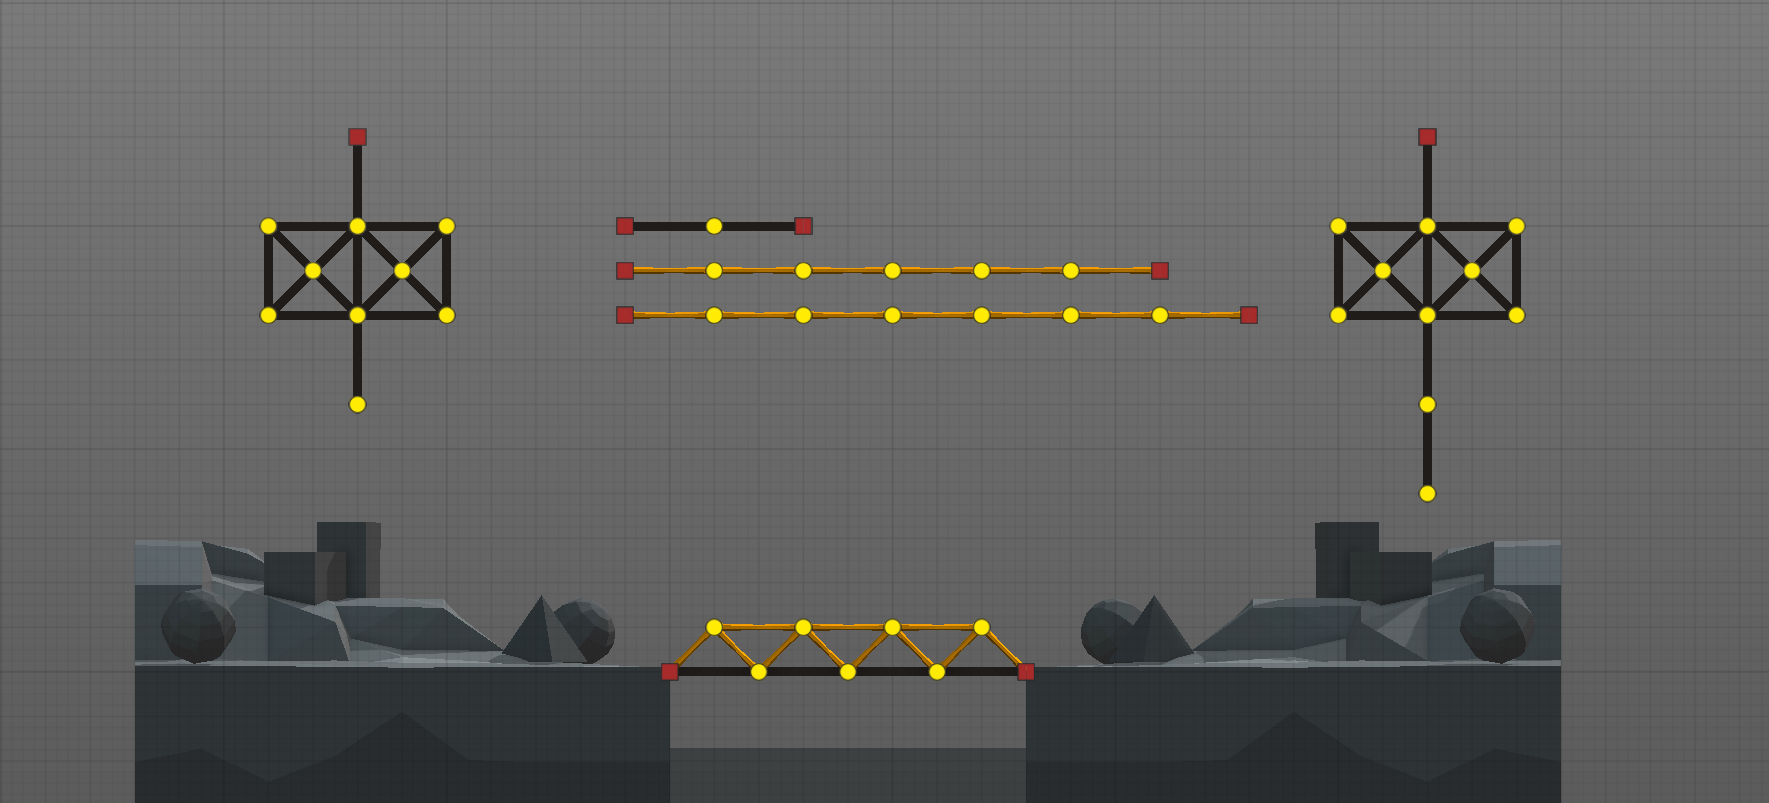
\includegraphics[width=\linewidth]{img/poly_tests.png}
    \end{minipage}\hfill
    \begin{minipage}{0.49\textwidth}
        \centering
        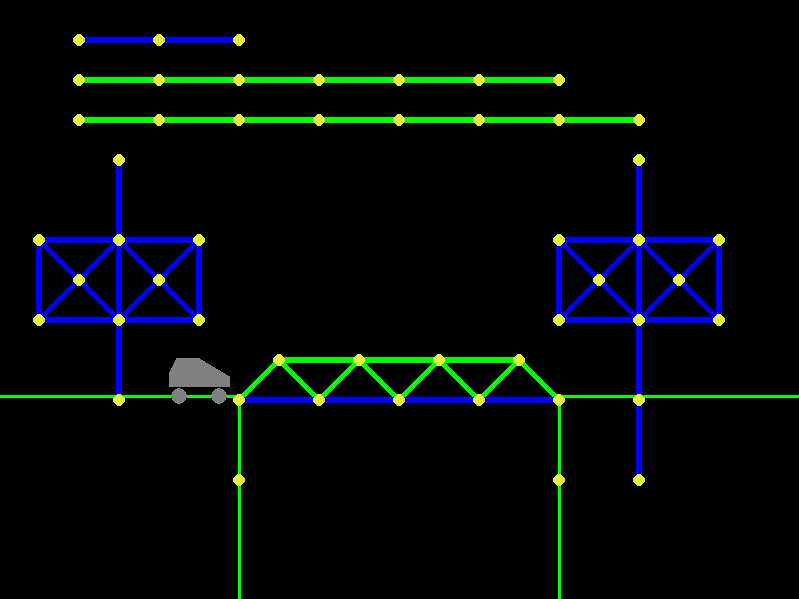
\includegraphics[width=\linewidth]{img/sim_tests.png}
    \end{minipage}
    \caption{Vizualizace testů ve hře polybridge (nalevo) a v simulaci (vpravo)}
    \label{fig:1}
\end{figure}


\xxx{simulace má 4 různé hyperparametry parametry, udělali jsme random search abychom splnili co nejvíce testů a aby simulace byla co nejstabilnější}


\xxx{podařilo se nám splnit jenom 5 testů z 6. může být problém v hře}

\subsection{Úrovně}

Jako testovací prostředí pro evoluční agloritmus jsme zvolili první 4 úrovně z původní hry. Více úrovní jsem kvůli jejich komplexitě nezahrnuli.

\begin{figure}[ht]
    \centering
    \begin{minipage}{0.49\textwidth}
        \centering
        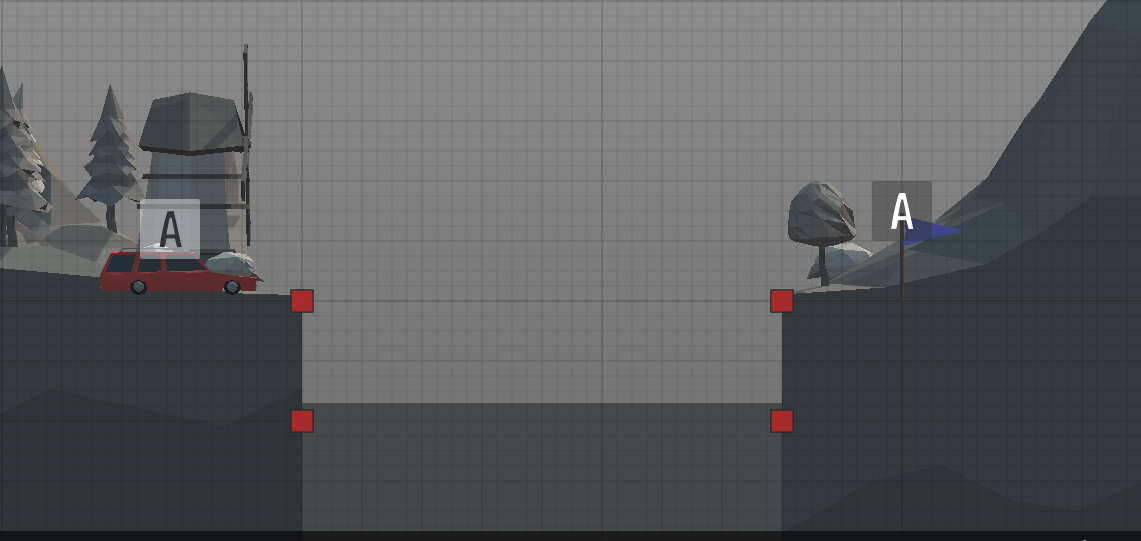
\includegraphics[width=\linewidth]{img/poly_lvl1.png}
    \end{minipage}\hfill
    \begin{minipage}{0.49\textwidth}
        \centering
        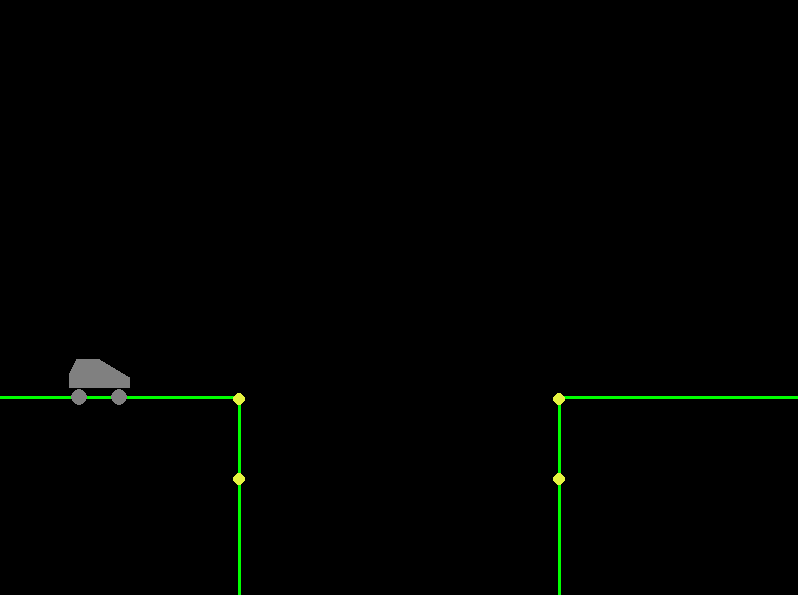
\includegraphics[width=\linewidth]{img/impl_lvl1.png}
    \end{minipage}
    \caption{Vizualizace první úrovně ve hře polybridge (vlevo) a v simulaci (vpravo)}
    \label{fig:2}
\end{figure}

\begin{figure}[ht]
    \centering
    \begin{minipage}{0.49\textwidth}
        \centering
        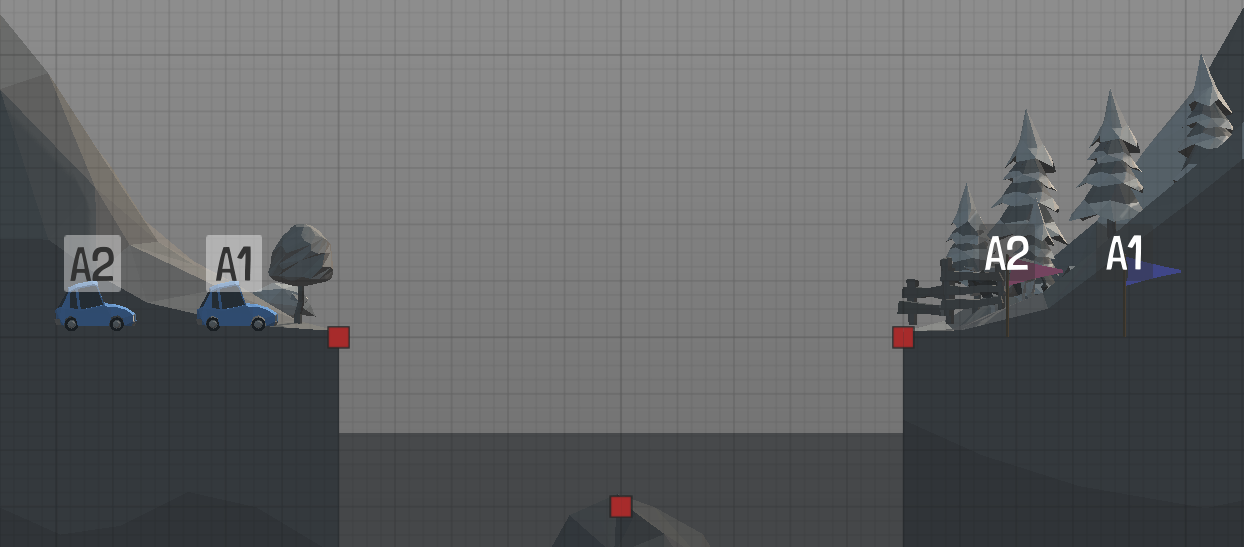
\includegraphics[width=\linewidth]{img/poly_lvl2.png}
    \end{minipage}\hfill
    \begin{minipage}{0.49\textwidth}
        \centering
        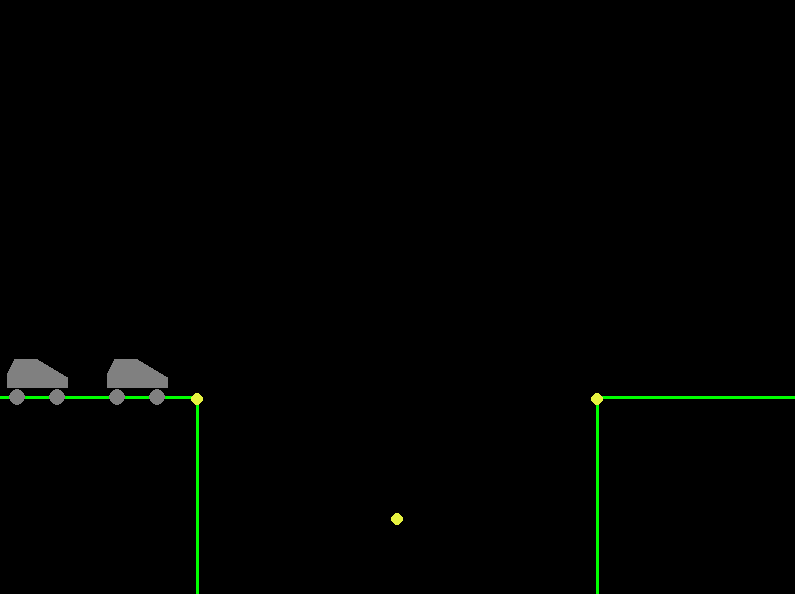
\includegraphics[width=\linewidth]{img/impl_lvl2.png}
    \end{minipage}
    \caption{Vizualizace druhé úrovně ve hře polybridge (vlevo) a v simulaci (vpravo)}
    \label{fig:3}
\end{figure}

\begin{figure}[ht]
    \centering
    \begin{minipage}{0.49\textwidth}
        \centering
        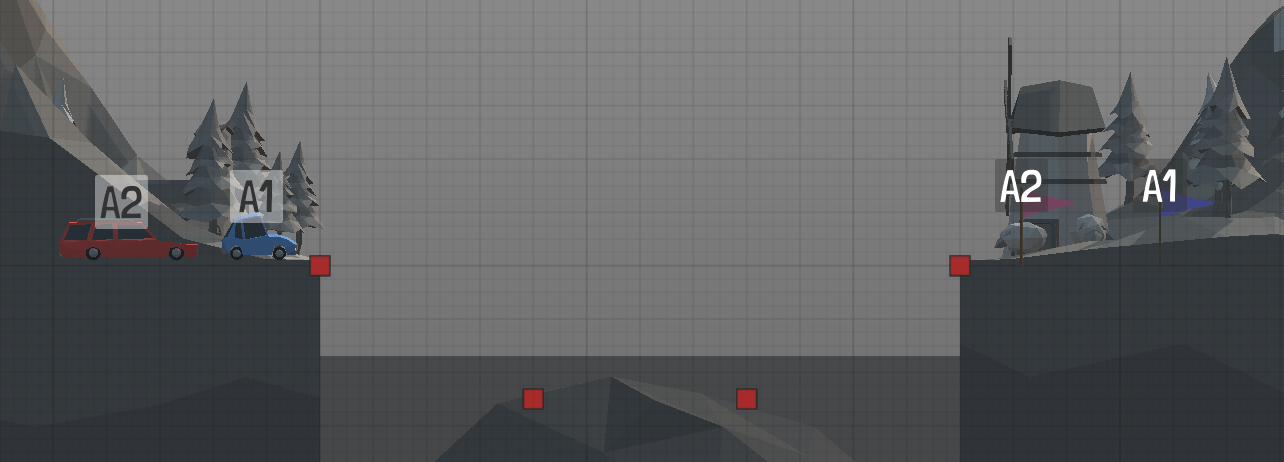
\includegraphics[width=\linewidth]{img/poly_lvl3.png}
    \end{minipage}\hfill
    \begin{minipage}{0.49\textwidth}
        \centering
        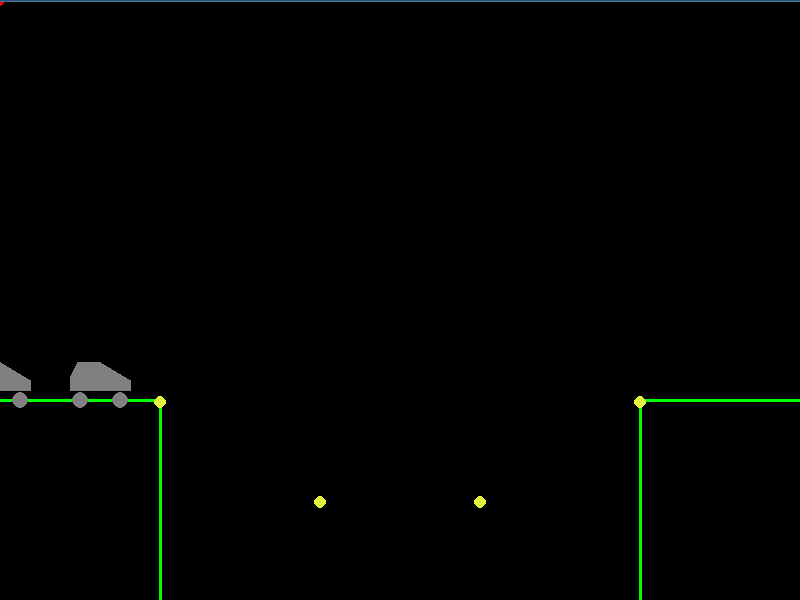
\includegraphics[width=\linewidth]{img/impl_lvl3.png}
    \end{minipage}
    \caption{Vizualizace třetí úrovně ve hře polybridge (nalevo) a v simulaci (vpravo)}
    \label{fig:4}
\end{figure}

\begin{figure}[ht]
    \centering
    \begin{minipage}{0.49\textwidth}
        \centering
        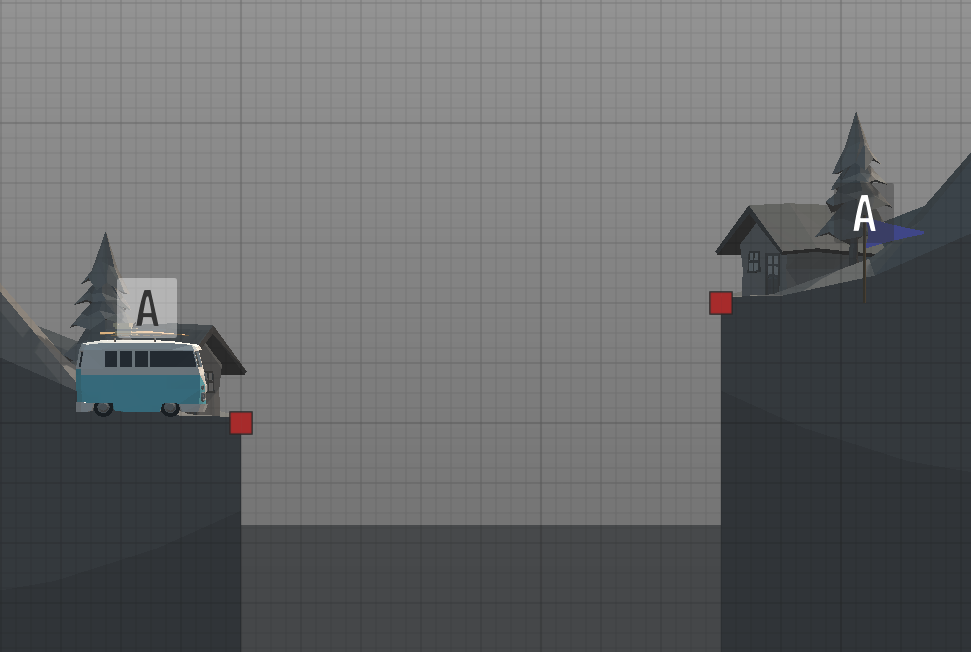
\includegraphics[width=\linewidth]{img/poly_lvl4.png}
    \end{minipage}\hfill
    \begin{minipage}{0.49\textwidth}
        \centering
        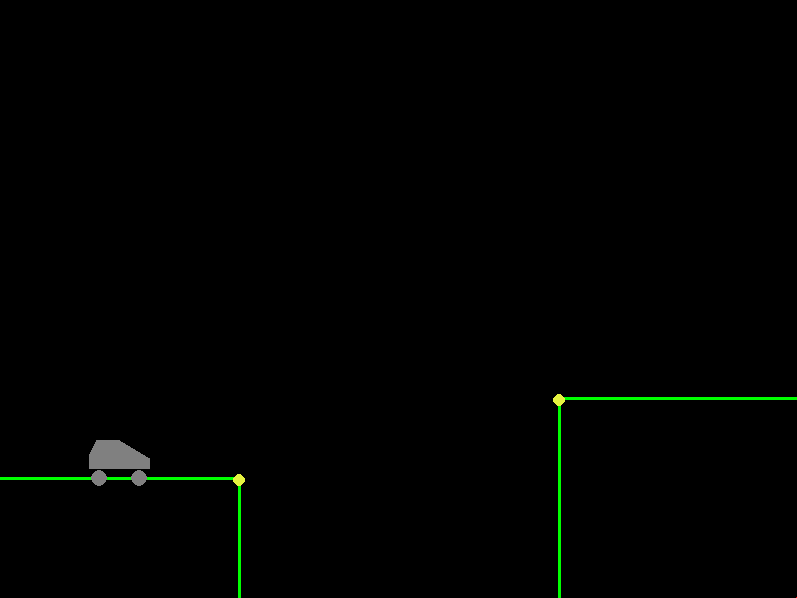
\includegraphics[width=\linewidth]{img/impl_lvl4.png}
    \end{minipage}
    \caption{Vizualizace čtvrté úrovně ve hře polybridge (nalevo) a v simulaci (vpravo)}
    \label{fig:5}
\end{figure}


\section{Aplikace evolučních algoritmů}

\xxx{Jak jsem udělal EA}

\xxx{můžů/mám sem dávat kousky kódu, z pythoní implementace? To by bylo možná snazší, než se to snažit popsat slovy}

Ve všech případech se snažíme optimalizovat dvě hodnoty a to jak daleko naše vozidlo dojelo a cenu mostu. V rámci algoritmu se tedy primárně snažíme maximalozovat $-dist = -||v - g||_2$ kde $v \in \R^2$ je pozice vozidla a $g \in \R^2$ je bod na druhé straně řeky a sekundárně $-cost$ kde $cost \in \N$ je cena mostu.

Naše fintess funcke $f$ bude tedu vždy udávaná dvojicí čísel $f(g) = (-dist, -cost)$ kde $g$ je gen mostu.

\subsection{Jednoduchý návrh}

Nejednušší návrh danému problému by mohl vypadat následovně. Reprezentace genu je vektor dvojic čísel $c \in \{([0, \dots, x_{max}] \times [0, \dots, y_{max}])\}^n$ kde $x_{max} \in \N$ a $y_{max} in \N$ je šířka a výška úrovně a vektor $t \in T^n$ kde $T$ je množina materiálů, které můžeme pužít (dřevo, vozovka, nic). Vektor $c$ představuje, serii kliknutí myši na obrazovku a $t$ jaký typ materiálu přidáme.

Jake mutaci jsme zvolili náhodné posunutí pozice kliknutí od $\pm 1$ s pravděpodobností $\frac{1}{n}$ a náhodnout změnu metariálu s pravděpodobností $\frac{1}{n}$.

Jako křížení jsme použili jednobodové křížení vektoru $c$  a $t$ podle stejně zvoleného náhodného bodu. Jako selekci jsme zvolili turnajovou selekci.

Jak můžeme vidět v experimentu (odkaz experiment), algortimu se nedaří stavět příliš kvalitní mosty. Domníváme se, že by tomu tak je z následujících důvodů.

\begin{itemize}
    \item Z principu reprezentace jedince je nepravděpodobné, aby vznikaly krátké hrany, které mohou být klíčové pro kvalitní řešení.
    \item I malá mutace na začátku genu může mít velký vliv na celkovou strukturu mostu.
    \item Křížení v naší reprezentaci nedává smysl.
    \item Fitness funkce nevrací dobrou zpětnou vazbu o kvalitě jedince \xxx{obrázek s porvnáním?}
\end{itemize}

\subsection{Polární kódování}

Kvůli tomu, jak jsme reprezentovali jedince v předchozím návrhu, je nepravděpodobné, že budou vznikat krátké hrany, které můžou být zásadní pro dobré řešení. To, že náhodně zvolíme blízko od od posledního kliknutí je méně pravděpodobné, než že zvolíme bod daleko. Proto jsme navrhli kódování genu, kde dvojce z vektoru $c$ představují délku a úhel přidaného materiálu $c \in \{([0, L_{max}] \times [0, 2 \pi])\}^n$ kde $L_{max}$ je maximální povolená délka materiálu. Vektor $t$ zůstává stejný jako v předchozím případě.

Vísledek běhu takto navrženého evolučního algoritmu můžeme vidět v experimentu (odkaz exepriment)

\subsection{Vylepšená fitness funkce}

Jedním z problémů, se kterým se náš současný návrh potýká je ten, že naše fitness funkce moc dobře nerozlišuje, jak je dané řešení kvalitní. Na obrázku (odkaz obrázek) můžeme vidět dva různé jednice, kteří mají stejnou fitness, a v kvalitě se značně liší.


\begin{figure}[ht]
    \centering
    \begin{minipage}{0.49\textwidth}
        \centering
        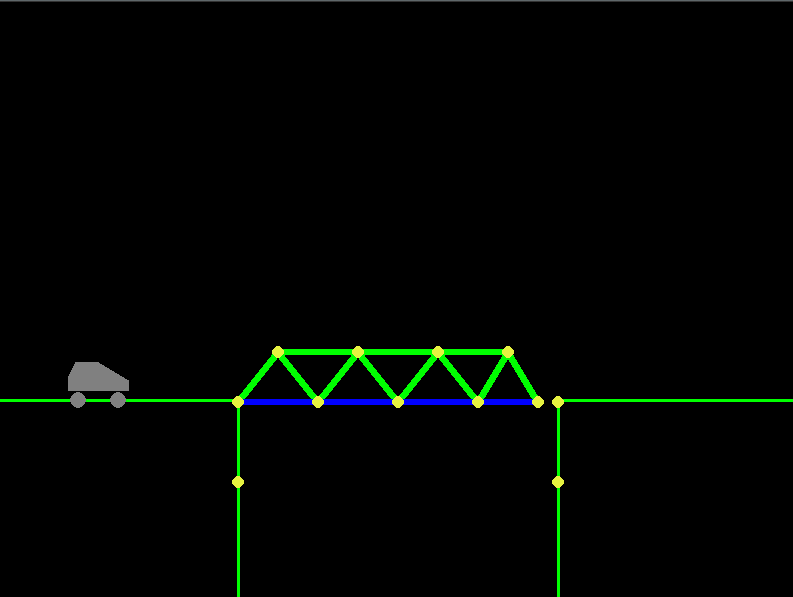
\includegraphics[width=\linewidth]{img/almost_good_bridge.png}
    \end{minipage}\hfill
    \begin{minipage}{0.49\textwidth}
        \centering
        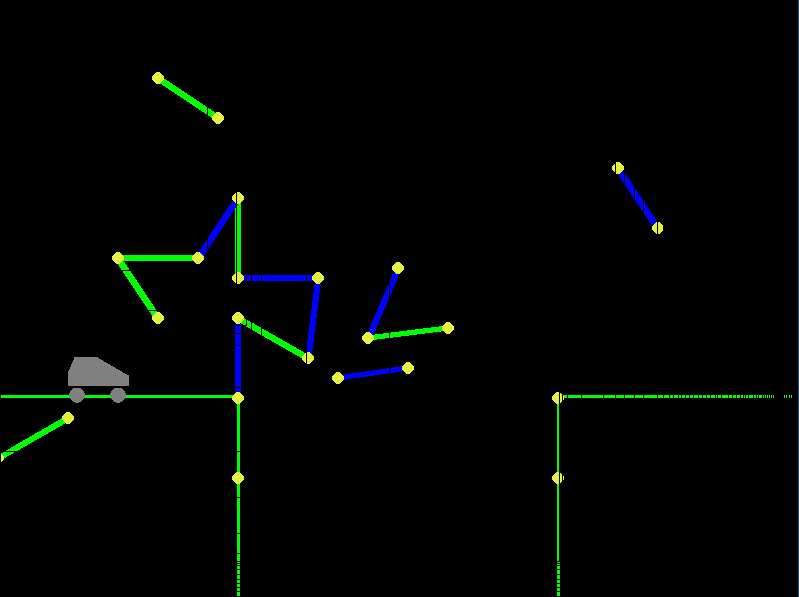
\includegraphics[width=\linewidth]{img/bad_bridge.png}
    \end{minipage}
    \caption{Dva mosty se stejnou fitness, ale rozdílných kvalit}
    \label{fig:5}
\end{figure}

Navrhli jsem proto několik rúzných penalizací, které můžeme do fitness zapojit.

\begin{itemize}
    \item Penalizace za umisťování materiálů, který se nespojí s další materíálem. Lépe propojený most by měl mít lepší stabilitu
    \item Penalizace za všechny kotvy, které jedince nepoužil v podobě vzdálenosti každého kliknutí ke všem nepoužitým kotvám. Most který používá více kotev by měl být stabilnější
    \item Penalizace za předčasně ukončenou simulaci. Simulace se předčasně ukončí pokud auto spadne, nebo pokud se dlouho nepohybuje
\end{itemize}

Fitness pak bude odpovídat $f(g) = (d_{min} + \alpha \cdot mat + \beta \cdot anch + \gamma \cdot term, cost)$, kde $\alpha, \beta, \gamma \in \R$ a $mat, anch, term$ jsou penalizace za nespojený materiál, nevyužité kontvy a předčasné ukončení.

\subsection{Měnící se fitness}

%Pro zlepšení zpětné vazby našeho systému se můzeme padsfsflnsdfkljasdfjsafdjlkdfsjkfdsajkdfsajk
\xxx{Udělám problém jednodušší. Dám břehy blíž k sobě, jakmile bude průměrná fitness dostatečně nízko, břehy trochu oddálím odkaz na IGA}

\subsection{Grafové kódování}

\xxx{Grafové kódování. Ukládám zvlášť vrcholy a hrany mostu}
\xxx{Popsané jak budou pak vypadat mutace a křížení}

\subsection{Lepší inicializace}

\xxx{Udělám stejnou init jako v článku (citace mosty)}
